\begin{frame} \frametitle{Voronoi Diagrams} \label{pg:definition}
\vspace{-0.24cm}

\begin{definition}
	\emph{Voronoi diagram} of set $S \subset \mathbb R^2$ of $n$ points is the subdivision
	of the plane into $n$ \emph{cells}, one for each site in $S$, with the property that
	a point $q$ lies in the cell corresponding to a site $s_i$ if and only if \vspace{-0.5cm}

	$$\mathrm{dist} (q, s_i) < \mathrm{dist} (q, s_j)$$ \vspace{-0.8cm}

	for each $s_j \in S$ with $j \ne i$.
\end{definition}

\begin{figure}[h] \centering
	\begin{subfigure}[t]{0.32\textwidth} \centering
		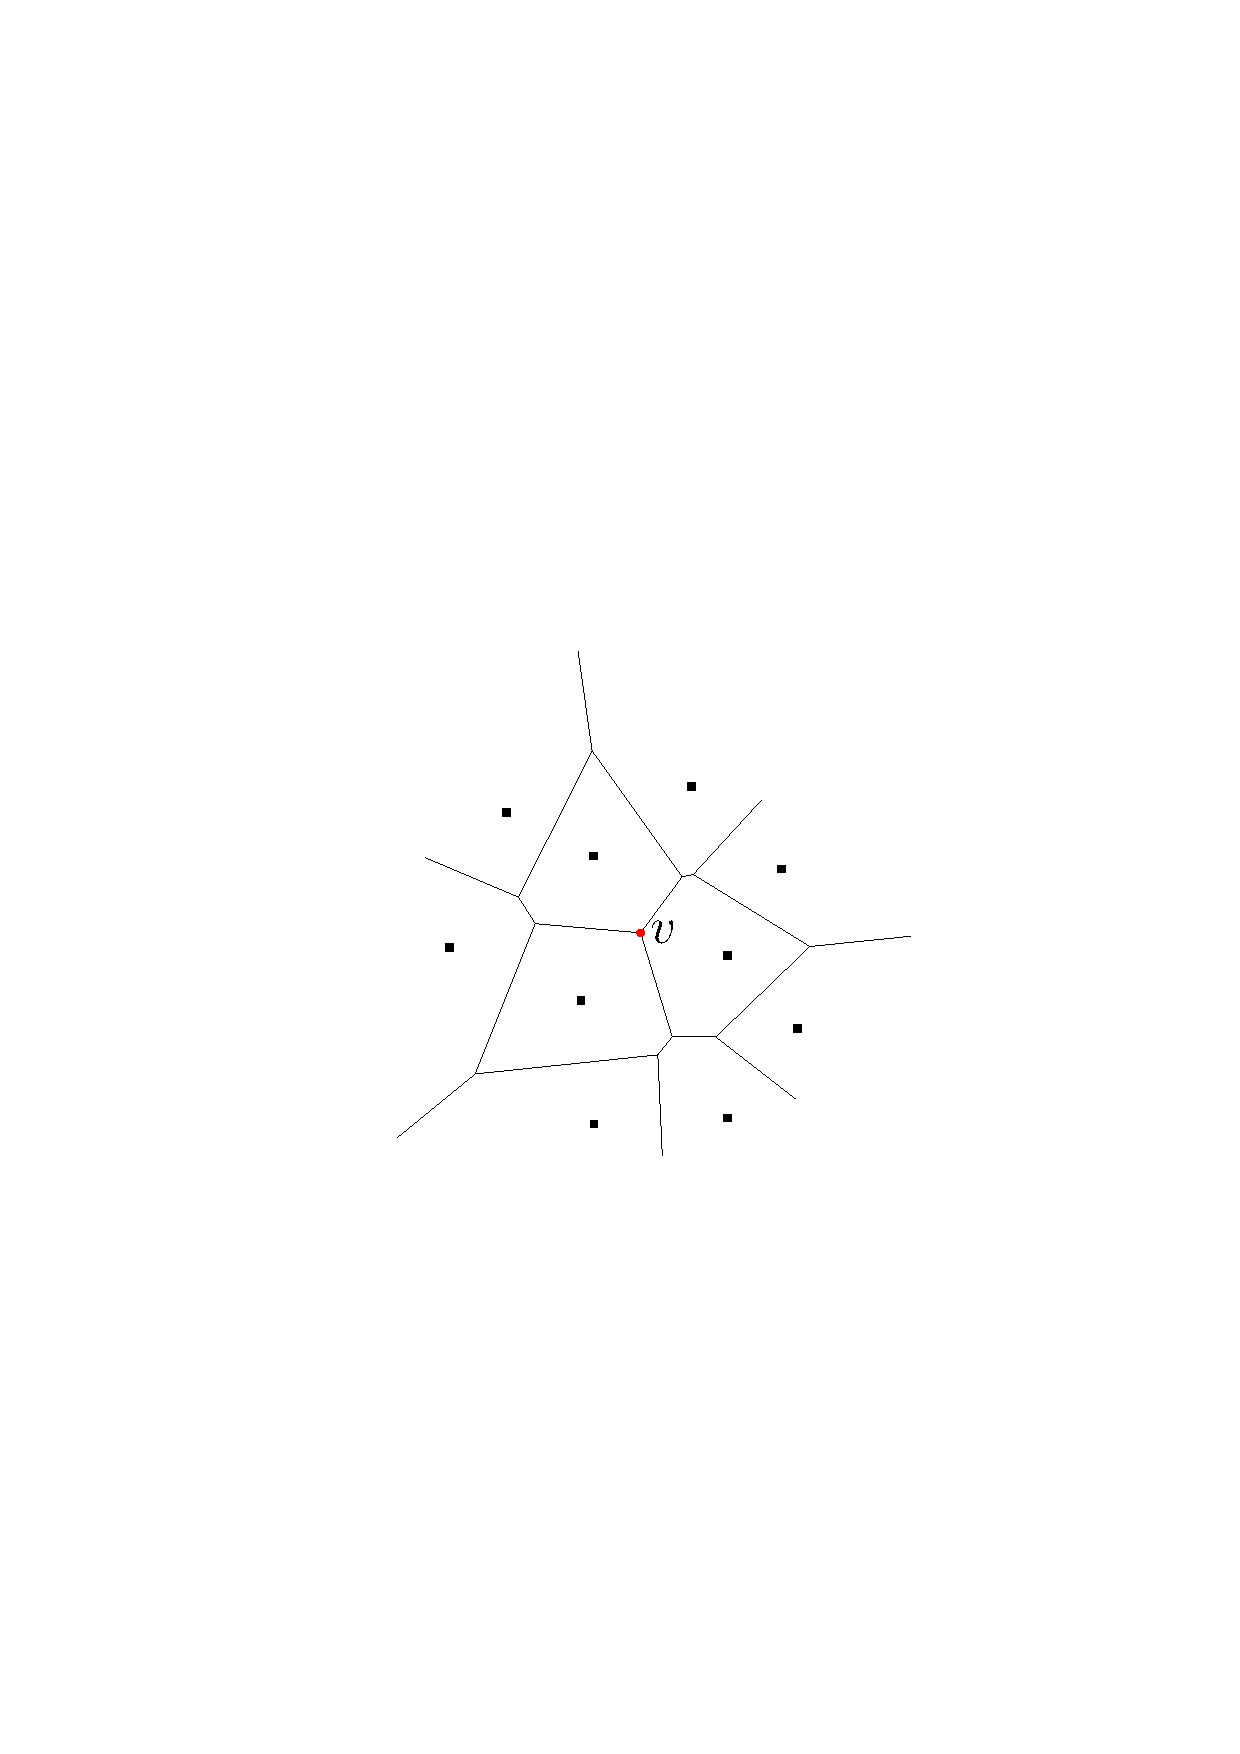
\includegraphics[width=3.7cm]{figs/voronoiDiagram}
	\end{subfigure} \quad
	\begin{subfigure}[t]{0.32\textwidth} \centering
		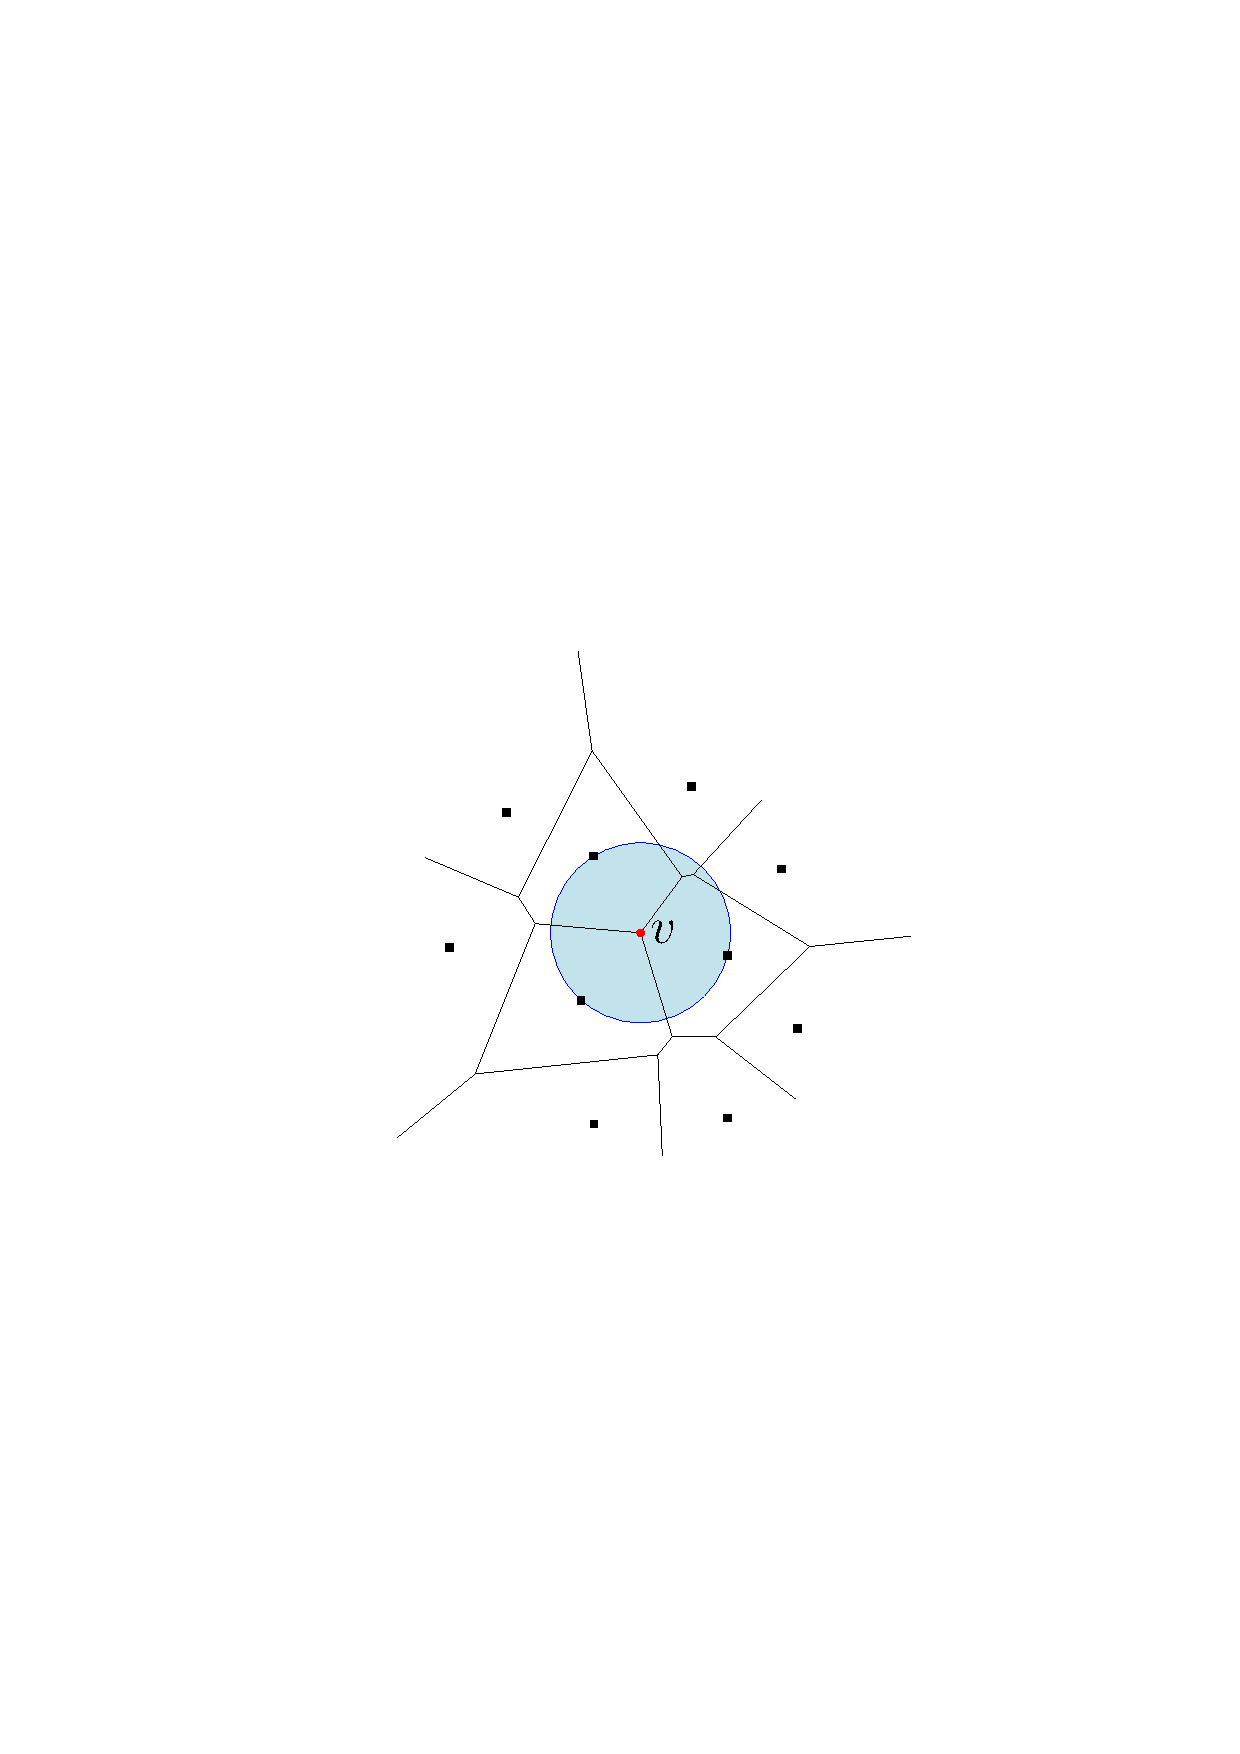
\includegraphics[width=3.7cm]{figs/voronoiCircle}
	\end{subfigure} \quad
\end{figure}

\end{frame}

\begin{frame} \frametitle{Algorithms for Voronoi Diagram}
\begin{enumerate}
	\item Calculate whole Voronoi diagram — $O(n \log n)$: sweep line, divide-and-conquer. \bigskip
	\item (And no better: sorting reduces to Voronoi.) \bigskip
	\item Update the diagram when a new site came — $O(n)$ — {\it literally any} possible way. \bigskip
	\item (And no better: {\it should draw en example here.} There can be that many changes.) \bigskip
	\item But what if we consider {\it the graph} of a diagram...
\end{enumerate}
\end{frame}

\begin{frame} \frametitle{Results today}
\begin{enumerate}
	\item $O(\sqrt{n})$, $\Omega(\sqrt{n})$ edge insertions / removals — even if the diagram is a tree. \bigskip
	
	This is in contrast to $O(n)$ geometric changes and $O(\log n)$ (amortised, existential) combinatorial changes in case of inserting in clockwise order. \bigskip

	\item {\it Algorithm} for insertion of sites in convex position, in arbitrary order — $O(\sqrt{n}\text{ polylog})$.
\end{enumerate}
\end{frame}

\begin{frame} \frametitle{Links and Cuts}
	{\it Link} is the addition of an edge, {\it cut} is the removal of an edge. We count only them. All other operations are thought to have no cost. For example, addition of a vertex. \ps

	How many links / cuts are there in our example?
\end{frame}

\begin{frame} \frametitle{Geometric vs Combinatorial Changes} \label{pg:combvsgeom}
\begin{center}
	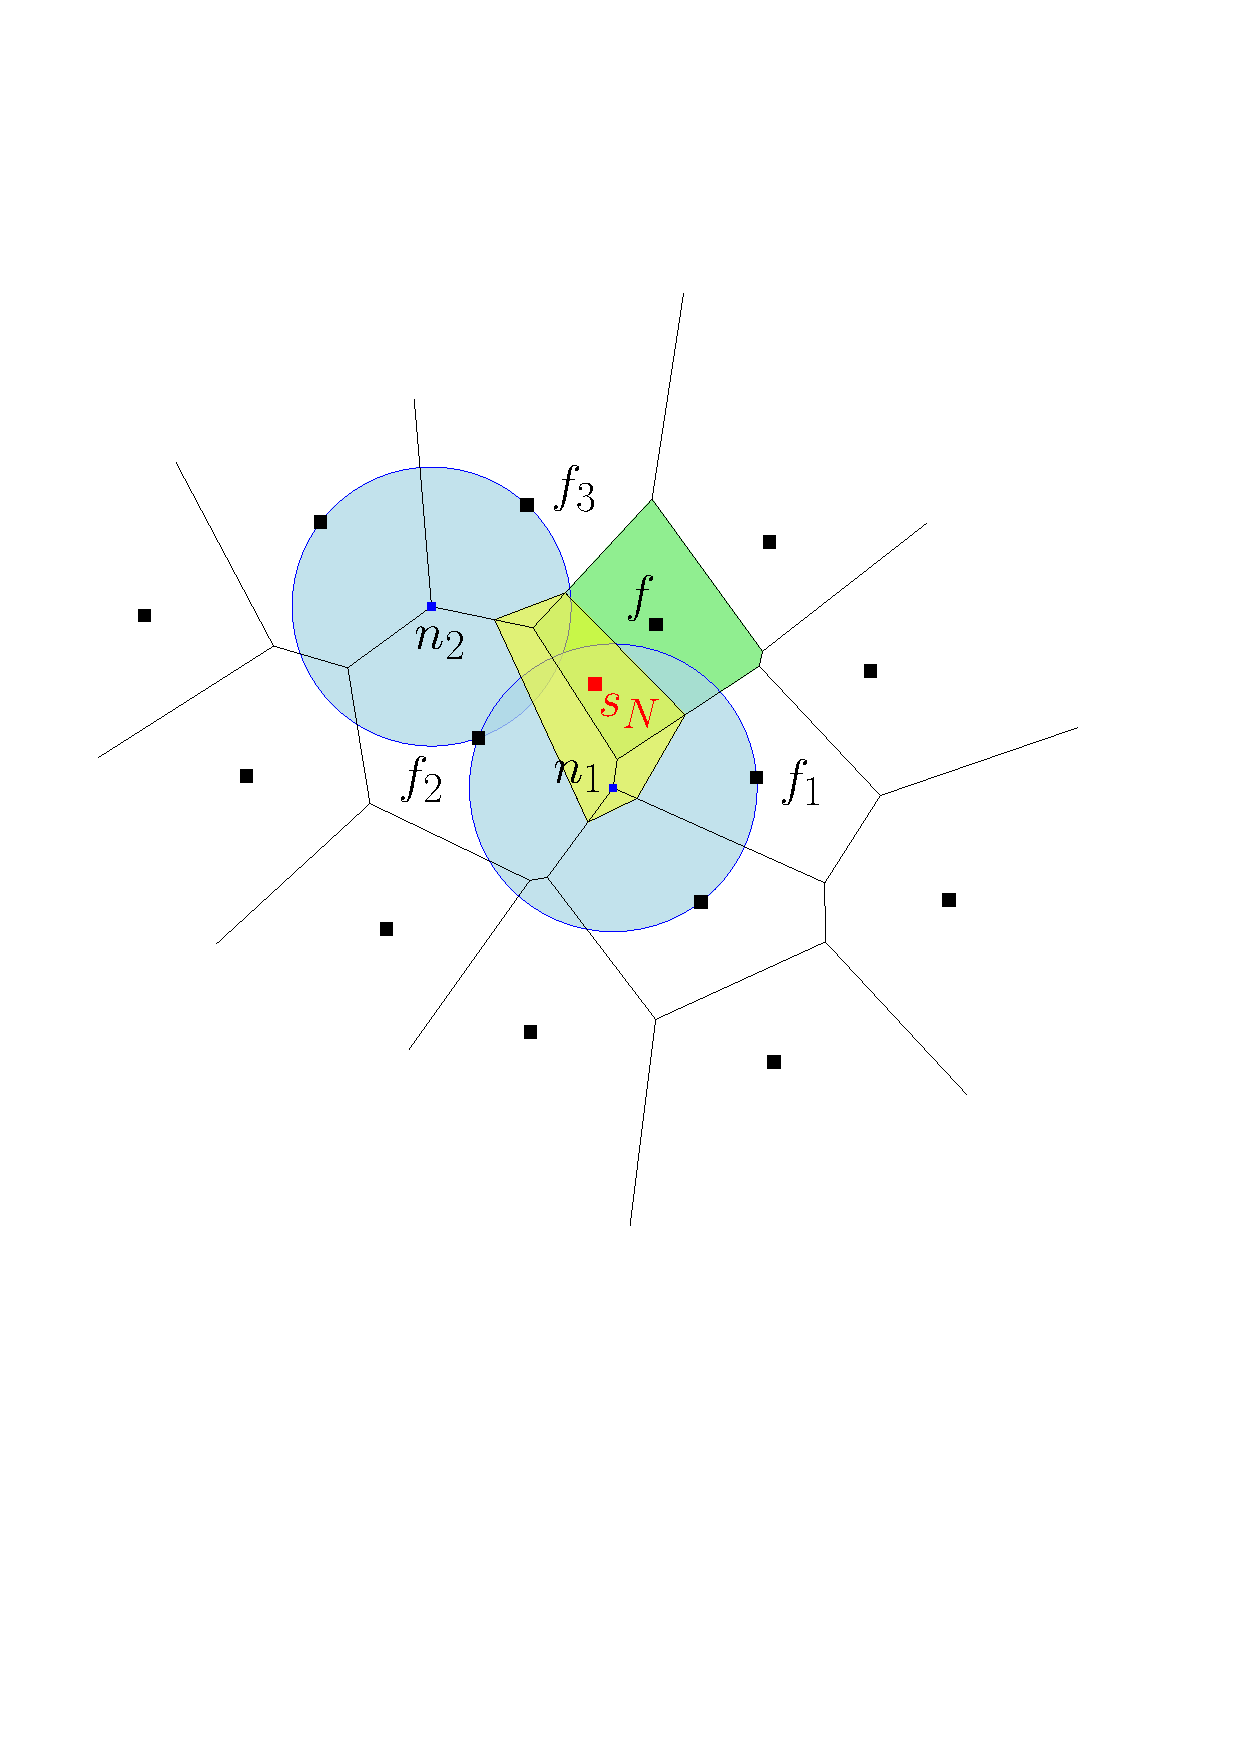
\includegraphics[width=7.4cm]{flarb/identChanges}
\end{center}
\end{frame}

\begin{frame} \frametitle{Chan's structure}
Can be used for:
	\begin{enumerate}
	\item Search of nearest neighbor;
	\item Reporting extreme point in given direction.
	\end{enumerate} \bigskip
Makes use of {\it shallow cuttings.} (Was presented at CG seminar.) Time complexity:
	\begin{enumerate}
	\item Insertion: $O(\log^3 n)$;
	\item Deletion: $O(\log^7 n)$ (improved to $^5$);
	\item Query: $O(\log^2 n)$.
	\end{enumerate}
\end{frame}

\begin{frame} \frametitle{Flarb}
\begin{figure}[h] \centering
	\begin{subfigure}[t]{0.31\textwidth}
	\centering
	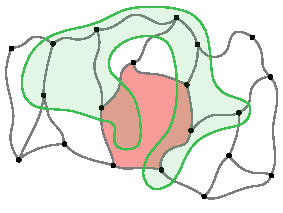
\includegraphics[scale=0.92]{flarb/1notflarb}
	\caption{This curve is not flarbable}
	\end{subfigure}
~
	\begin{subfigure}[t]{0.31\textwidth}
	\centering
	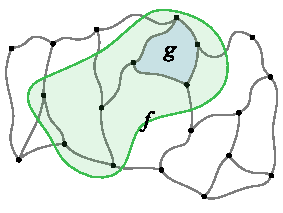
\includegraphics[scale=0.92]{flarb/2flarb}
	\caption{This curve is flarbable}
	\end{subfigure}
~
	\begin{subfigure}[t]{0.31\textwidth}
	\centering
	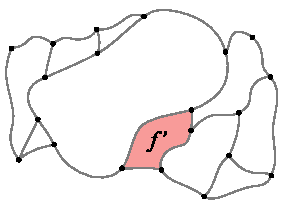
\includegraphics[scale=0.92]{flarb/3afterflarb}
	\caption{Result of applying flarb operation}
	\end{subfigure}
\end{figure} \medskip

Fleeq-edges:  those intersecting $\mC$. Note that in a real Voronoi diagram there can be no such cells as $g$.
\end{frame}